\documentclass[a4paper,12pt]{article}
\usepackage[utf8]{inputenc}
\usepackage{listings}
\usepackage{float}
\usepackage[margin=1in]{geometry}
\setlength\parindent{0pt}
\usepackage{xcolor}
\usepackage{graphicx}
\definecolor{dkgreen}{rgb}{0,0.6,0}
\definecolor{dred}{rgb}{0.545,0,0}
\definecolor{dblue}{rgb}{0,0,0.545}
\definecolor{lgrey}{rgb}{0.9,0.9,0.9}
\definecolor{gray}{rgb}{0.4,0.4,0.4}
\definecolor{darkblue}{rgb}{0.0,0.0,0.6}
\lstdefinelanguage{python}{
      backgroundcolor=\color{lgrey},  
      basicstyle=\footnotesize \ttfamily \color{black} \bfseries,   
      breakatwhitespace=false,       
      breaklines=true,               
      captionpos=b,                   
      commentstyle=\color{dkgreen},   
      deletekeywords={...},          
      escapeinside={\%*}{*)},                  
      frame=single,                  
      language=C++,                
      keywordstyle=\color{purple},  
      morekeywords={BRIEFDescriptorConfig,string,TiXmlNode,DetectorDescriptorConfigContainer,istringstream,cerr,exit}, 
      identifierstyle=\color{black},
      stringstyle=\color{blue},      
      numbers=right,                 
      numbersep=5pt,                  
      numberstyle=\tiny\color{black}, 
      rulecolor=\color{black},        
      showspaces=false,               
      showstringspaces=false,        
      showtabs=false,                
      stepnumber=1,                   
      tabsize=5,                     
      title=\lstname,                 
    }
    
%opening
\title{CS325 Homework 2}
\author{Kabir Kang, Paul Ely, Jason Dorweiler}

\begin{document}

\maketitle

\section*{Recursive Function}
\textbf{Describe the solution to the maximum subarray problem recursively and mathematically based on the above idea.}

The given idea was: \emph{The maximum subarray either uses the last element in the input array, or it doesn't}. For an array A with n elements, a recursive function to solve this problem would find the maximum value of all subarrays up to n. For each subarray, it would test whether the next element should be included in the maximum sum or whether it should not.

So, let A be an array with n elements. Then let MaxSum(k) be the maximum sum of all subarrays up to and ending at j. Then the maximum subarray value can be found by taking max( MaxSum(k-1) + A[k], A[k] ).



\section*{Pseudocode - DP Solution}
  \begin{lstlisting}[language=python,caption={pseudo code for DP algorithm},mathescape]
MaxSubArray(array):
    maxSum = -$\infty$
    tempSum = 0
    for i in array:
    	if tempSum > 0:
    		tempSum = tempSum + i
    	else:
    		tempSum = i
    	maxSum = np.maximum(maxSum, tempSum)
    return maxSum	
  \end{lstlisting}


\section*{Running Time}

The running time for this algorithm is $\theta(n)$. The algorithm only loops from 0 to n once, performing a number of constant-time operations per iteration. It will always run from 0 to n, thus giving a $\theta(n)$ running time.  The calculated running time for the dynamic algorithm based on the slope of our log-log plot is 0.98 which shows our assumptions are correct.  The run time for the $n\log(n)$ algorithm came out out to 1.10 based on the slope of our log-log plot. 

\section*{Theoretical Correctness}

MaxSubArray will return the maximum value contiguous subarray for some array $A$ with $n$ elements, where $n>0$. It does so by saving the maximum subarray value and building up from 0 to n. 

\textbf{Base case}: The base case is when $n=1$. Then the value of the maximum subarray is $A[n]$.

\textbf{Proof}: Assume that the algorithm is correct for $1\leq n \leq k$. Now consider adding another element to the array. There are two cases:

\begin{itemize}


\item Case 1: running sum is $> 0$. In this case, the next element is added to the running sum.

\item Case 2: the running sum is $<= 0$. In this case, the running sum is set equal to the next element. 

\end{itemize}

The maximum value is then set to the maximum of either the previous maximum or the running sum. By the inductive hypothesis, we know that the previous maximum sum was the maximum value for the subarray up to $k$. Therefore the algorithm correctly returns the maximum subarray.


\pagebreak
 
\begin{figure}[h!]
\centering
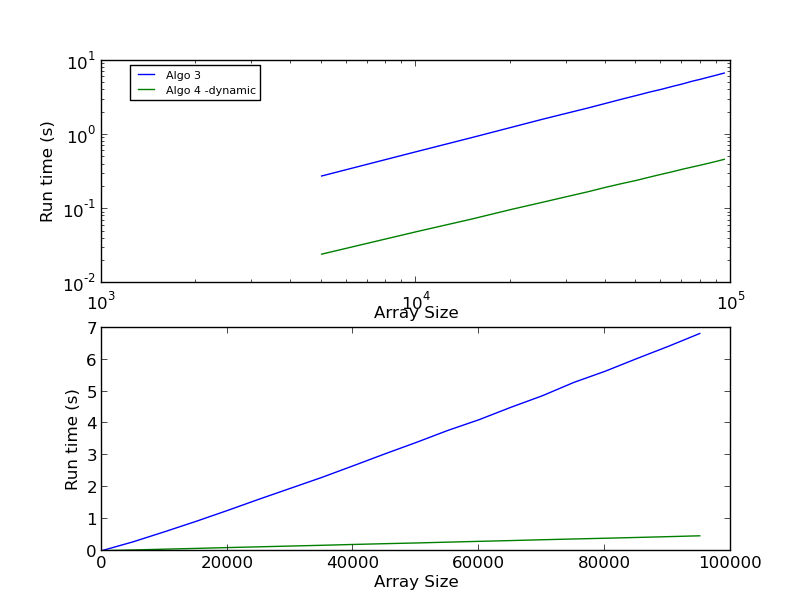
\includegraphics[width=0.8\textwidth]{algo4runtime}
\caption{Plot of the dynamic algorithm (green) and the $n\log(n)$ algorithm from homework1}
\end{figure} 

\section*{Compare}


**Notes: delete this later**** I don't see a lot of downsides to the dynamic version?? maybe there aren't any?  Algo 3 runs slower and also needs to store its result in another array which increases the space complexity. ***
\end{document}